% THIS TEMPLATE IS A WORK IN PROGRESS

\documentclass{article}
\usepackage{graphicx}
\usepackage{hyperref}
\usepackage{fancyhdr}
\usepackage{float}

% FOR CODE
\usepackage{listings}
\usepackage{xcolor}

\usepackage{amsmath}

\definecolor{codegreen}{rgb}{0,0.6,0}
\definecolor{codegray}{rgb}{0.5,0.5,0.5}
\definecolor{codepurple}{rgb}{0.58,0,0.82}
\definecolor{backcolour}{rgb}{0.95,0.95,0.92}

\lstdefinestyle{mystyle}{
    backgroundcolor=\color{backcolour},   
    commentstyle=\color{codegreen},
    keywordstyle=\color{magenta},
    numberstyle=\tiny\color{codegray},
    stringstyle=\color{codepurple},
    basicstyle=\ttfamily\footnotesize,
    breakatwhitespace=false,         
    breaklines=true,                 
    captionpos=b,                    
    keepspaces=true,                 
    numbers=left,                    
    numbersep=5pt,                  
    showspaces=false,                
    showstringspaces=false,
    showtabs=false,                  
    tabsize=2
}

\lstset{style=mystyle}
% 

\fancypagestyle{firstpage}{%
  \lhead{CAP6610 Home Work 2}
  \rhead{Akash Gajjar}
}

\begin{document}
\thispagestyle{firstpage}

\section*{Question 1 Answer}

For a boolean function on 5 variables, the Karnaugh map has 32 cells, corresponding to the $2^{5} = 32$ possible input combinations. Each cell can be either 0 or 1, so there are $2^{32}$ possible boolean functions on 5 variables.

The maximum number of minterms in the Karnaugh map of a boolean function on 5 variables is 16. This is because if a boolean function on 5 variables has more than 16 minterms (i.e., more than 16 ones in its Karnaugh map), then at least one pair of adjacent cells can be grouped together to form a larger group of multiple cells that can be covered by a single gate. Therefore, the maximum number of gates required in a single hidden layer to implement a boolean function with 5 inputs is 16.

However, it's worth noting that constructing a network with 16 gates that can implement a complex function can be difficult in practice, and a more efficient network may require fewer gates. Increasing the number of layers in the network can allow for a more efficient implementation of the function. By adding additional layers to the network, the gates in each layer can be used to combine the output of gates in the previous layer, creating a hierarchical structure that can represent more complex functions with fewer gates. Any boolean function on $n$ variables can be expressed as a composition of boolean functions on two variables using the Boolean Algebra. We can construct the network like a binary tree, that would result in a tree with total 4 nodes and $\log_{2} 5 \approx 3$ layers. This is what the network would look like 

\begin{figure}[H]
  \centering
  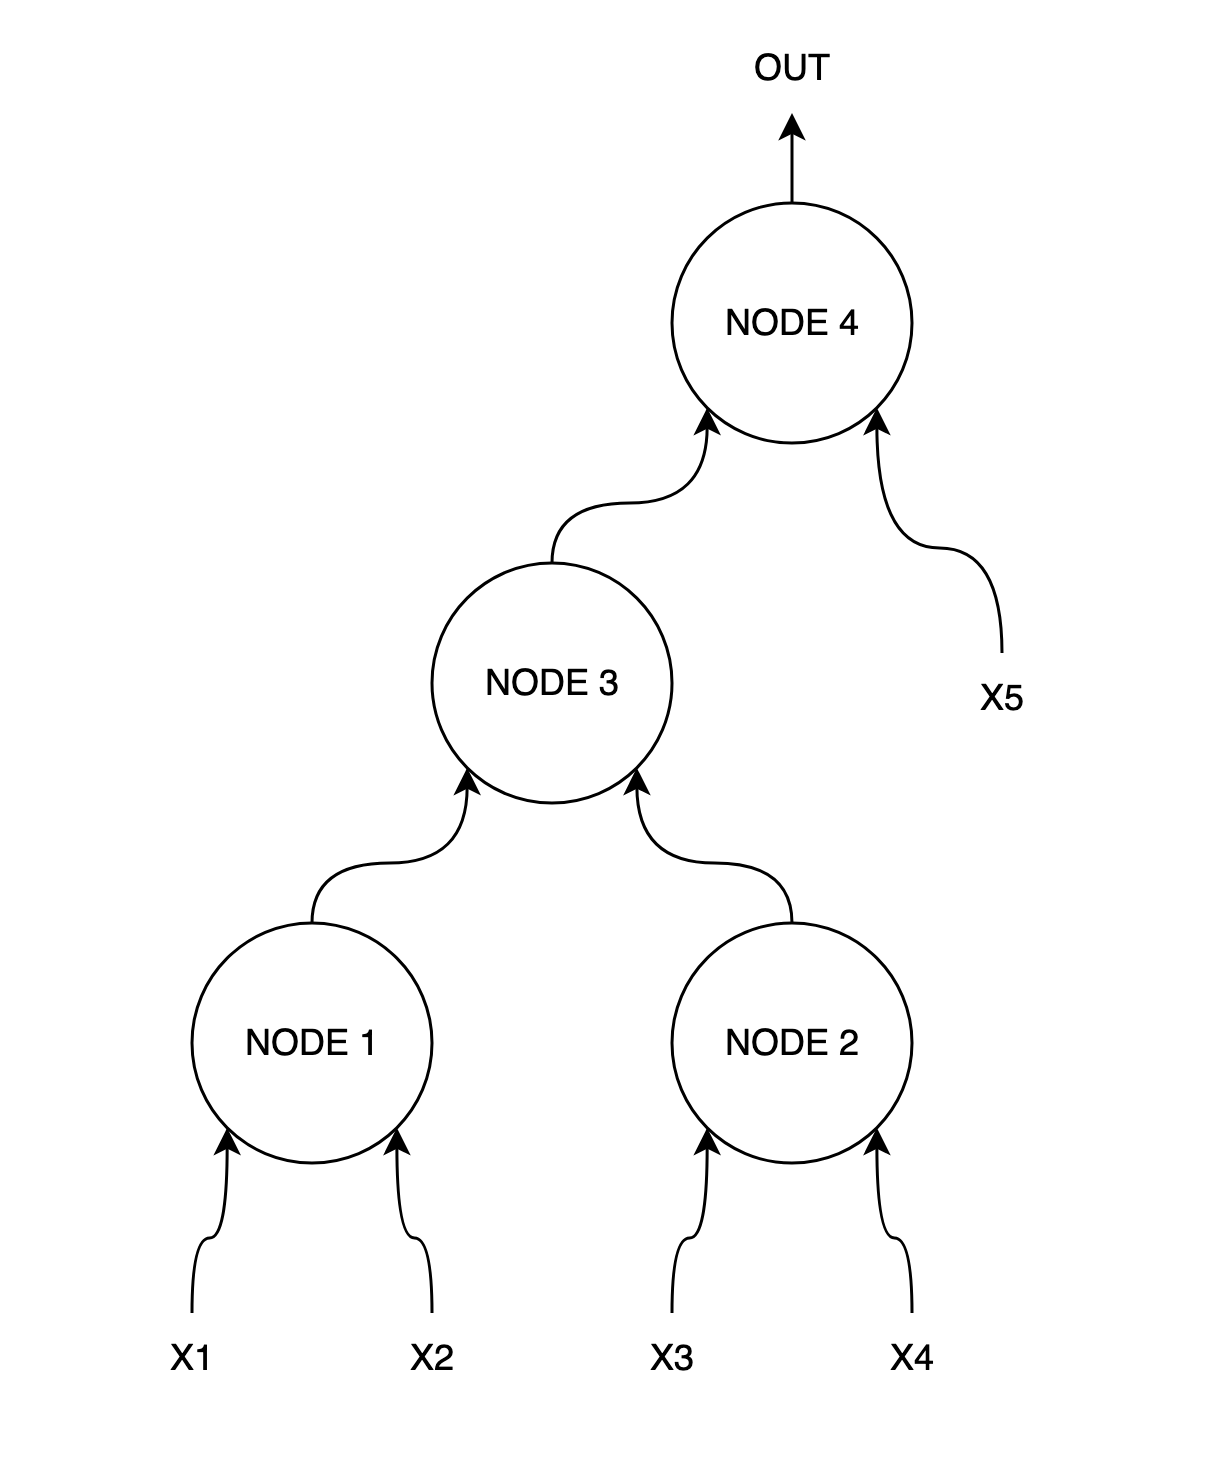
\includegraphics[width=2.5in]{images/network.png}
\end{figure}

Depending on the boolean function, there may be a case where the K-map reduces the whole function to a single gate.

\section*{Question 2 Answer}
Here is the implementation code
\lstinputlisting[language=Python]{code.py}

As we increase the number of epochs, the accuracy of the model increases. For example, for 10 epochs the accuracy is around $65\%$, for 100 epochs the accuracy is around $80\%$, and for 1000 epochs the accuracy is around $95\%$. Learning rate and the threshold at which we convert the output to label also changes the accuracy of the model. I have found that initializing the weights with values from the uniform distribution $[-1,1]$ works well.
\section*{Question 3 Answer}

The output can be expressed as the following function,

\begin{displaymath}
    f(x_1,\dots,x_n) = 
    \begin{cases} 
        \mbox{1,} & \mbox{if } \sum x_i < \frac{n}{2}, i = \{1\dots n\} \\ 
        \mbox{0,} & \mbox{otherwise} 
    \end{cases} 
\end{displaymath}
%
The perceptron models the function,
\begin{displaymath}
    \hat{f}(x_1,\dots,x_n) = threshold(\omega^T X + b)
\end{displaymath}

where,
\begin{displaymath}
    threshold(x) = 
    \begin{cases}
        \mbox{1,} & \mbox{if } x > 0 \\
        \mbox{0,} & \mbox{otherwise}
    \end{cases}
\end{displaymath}

and,
\begin{displaymath}
    X = \begin{bmatrix}x_1\\ . \\ . \\x_n\end{bmatrix},\\
    \omega = \begin{bmatrix}\omega_1\\ . \\ . \\\omega_n\end{bmatrix} \\
    b = \mbox{bias}
\end{displaymath}
%
If we initialize all the weights ($\omega_1,\dots,\omega_n$) as -1 and bias as $\frac{n}{2}$ then the $\hat{f}$ would return 1 if more of  $x_i$ have value 0 than value 1, otherwise returns 0.

\section*{Question 4 Answer}

Here we have our error defined as mean squared error,

\begin{equation}
\label{eq:1}
    E = \frac{1}{2}(t - o)^2
\end{equation}

where,
\begin{displaymath}
    t = \mbox{real valued output}
\end{displaymath}
\begin{equation}
\label{eq:2}
    o = \mbox{artificial neuron output} = e^{net}
\end{equation}
\begin{equation}
\label{eq:3}
    net = wx, \mbox{where } w = \mbox{weight, } x = \mbox{input}
\end{equation}
%
and the weight update would be given by the equation
\begin{displaymath}
    w_i \leftarrow w_i + \Delta w
\end{displaymath}
\begin{displaymath}
    \Delta w = - \eta \frac{dE}{dw}
\end{displaymath}
%
and we can rewrite $\frac{dE}{dw}$ as
\begin{equation}
    \label{eq:4}
    \frac{dE}{dw} = \frac{dE}{do} \frac{do}{dnet} \frac{dnet}{dw}
\end{equation}
%
from \eqref{eq:1} we get,
\begin{equation}
    \label{eq:4}
    \frac{dE}{do} = o - t
\end{equation}
%
from \eqref{eq:2} we get,
\begin{equation}
    \label{eq:5}
    \frac{do}{dnet} = o
\end{equation}
%
from \eqref{eq:3} we get,
\begin{equation}
    \label{eq:6}
    \frac{dnet}{dw} = x
\end{equation}
%
now plugging in these values to \eqref{eq:4} we get,

\begin{displaymath}
    \frac{dE}{dw} = (o - t) \times o \times x
\end{displaymath}
%
so the weight update equation would be
\begin{displaymath}
    w \leftarrow w + \eta ox(t - o)
\end{displaymath}

where w = weight, $\eta$ is the learning rate, $x$ is the input, $t$ is the real valued output, $o$ is the output from the artificial neuron.

I am not including the bias weight since the question asks to model an artificial neuron with a single weight.
\end{document}
